%%%%%%%%%%%%%%%%%%%%%%%%%%%%%%%%%%%%%%%%%%%%%%%%%%%%%%%%%%%%%%%%%%%%%%%%%%%%%%%%%%
\begin{frame}[fragile]\frametitle{}
\begin{center}
{\Large Cypher}
\end{center}
\end{frame}


%%%%%%%%%%%%%%%%%%%%%%%%%%%%%%%%%%%%%%%%%%%%%%%%%%%%%%%%%%%
\begin{frame}[fragile]\frametitle{Introduction}
A pattern matching query language made for graphs

\begin{itemize}
\item Declarative: say, what you want? and not how to search for the answer (Imperative)
\item Expressive
\item Pattern-Matching : ASCI Art
\end{itemize}

\end{frame}



%%%%%%%%%%%%%%%%%%%%%%%%%%%%%%%%%%%%%%%%%%%%%%%%%%%%%%%%%%%
\begin{frame}[fragile]\frametitle{Use Case}

Movie Dataset

\begin{itemize}
\item The graph contains nodes with the labels Person and Movie. 
\item Person nodes have several types of relationships to Movie nodes. 
\item A Person node can have a FOLLOWS relationship to another Person node.
\end{itemize}


\begin{center}
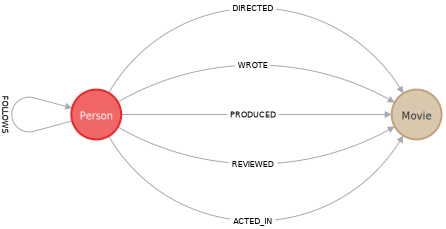
\includegraphics[width=0.5\linewidth,keepaspectratio]{neo4j62}
\end{center}	  


{\tiny (Ref: Introduction to cypher fundamentals  - neo4j)}

\end{frame}

%%%%%%%%%%%%%%%%%%%%%%%%%%%%%%%%%%%%%%%%%%%%%%%%%%%%%%%%%%%
\begin{frame}[fragile]\frametitle{Representation}


\begin{itemize}
\item Nodes are represented in round brackets \lstinline|()|
\item Relationships are represented as arrow with its label in square bracket in between \lstinline|-[]->|
\item \lstinline|(variable:label)|
\end{itemize}


\begin{center}
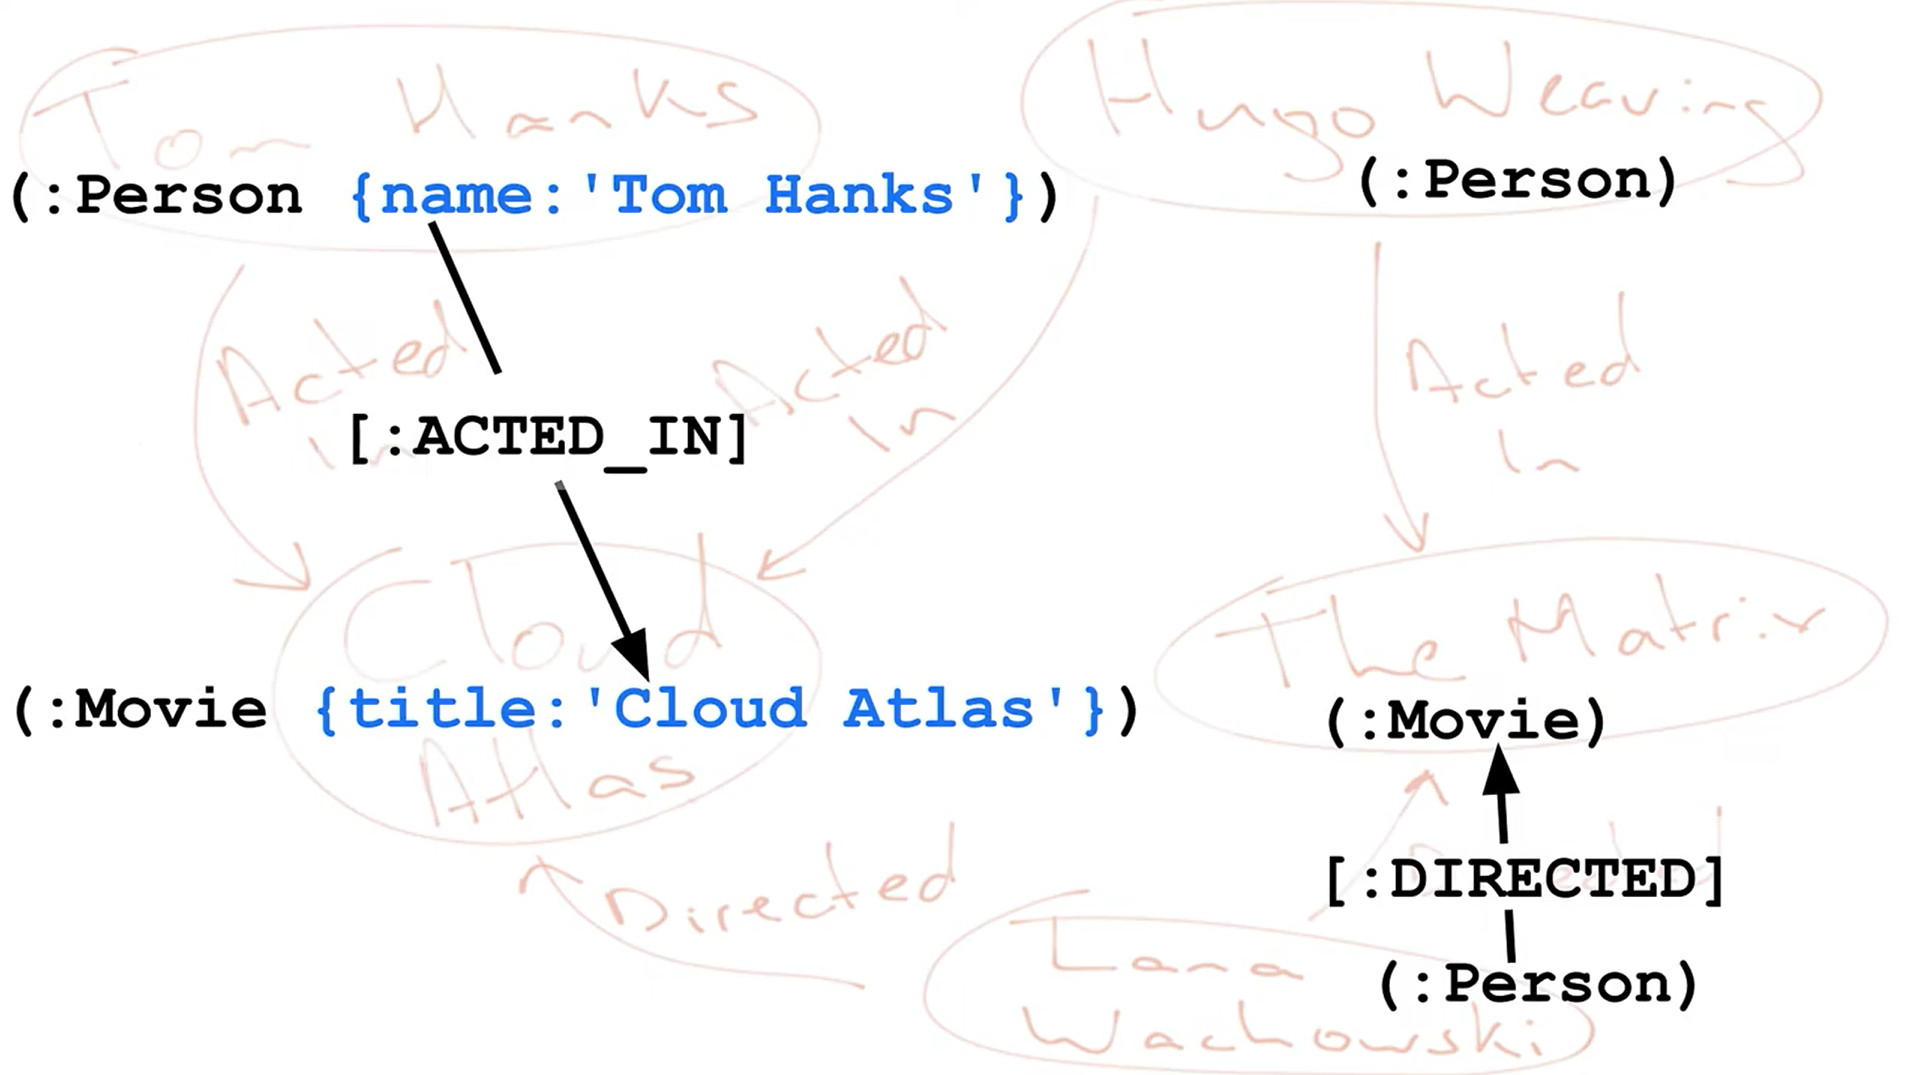
\includegraphics[width=0.5\linewidth,keepaspectratio]{neo4j63}
\end{center}	  


{\tiny (Ref: Introduction to cypher fundamentals  - neo4j)}

\end{frame}

%%%%%%%%%%%%%%%%%%%%%%%%%%%%%%%%%%%%%%%%%%%%%%%%%%%%%%%%%%%%%%%%%%%%%%%%%%%%%%%%%%
\begin{frame}[fragile]\frametitle{}
\begin{center}
{\Large Reading}
\end{center}
\end{frame}


%%%%%%%%%%%%%%%%%%%%%%%%%%%%%%%%%%%%%%%%%%%%%%%%%%%%%%%%%%%
\begin{frame}[fragile]\frametitle{Basic Syntax}

\begin{center}
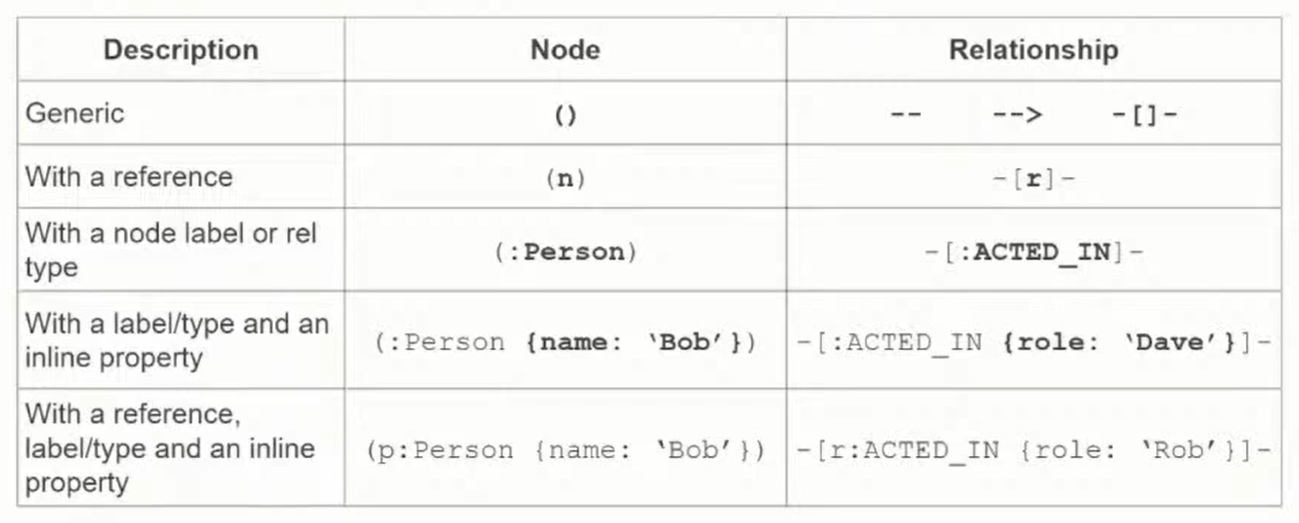
\includegraphics[width=\linewidth,keepaspectratio]{neo4j9}
\end{center}	  


{\tiny (Ref: Introduction to Neo4j - a hands-on crash course  - neo4j)}

\end{frame}

%%%%%%%%%%%%%%%%%%%%%%%%%%%%%%%%%%%%%%%%%%%%%%%%%%%%%%%%%%%
\begin{frame}[fragile]\frametitle{Retrieval}


\begin{itemize}
\item Pattern specification for MATCH command, to retrieve data in graph.
\item Find and return person $p$ and movie $m$
\item First finds $p$ with given name, then goes to all relationships with given type and then finds $m$ which matches given title.
\end{itemize}


\begin{center}
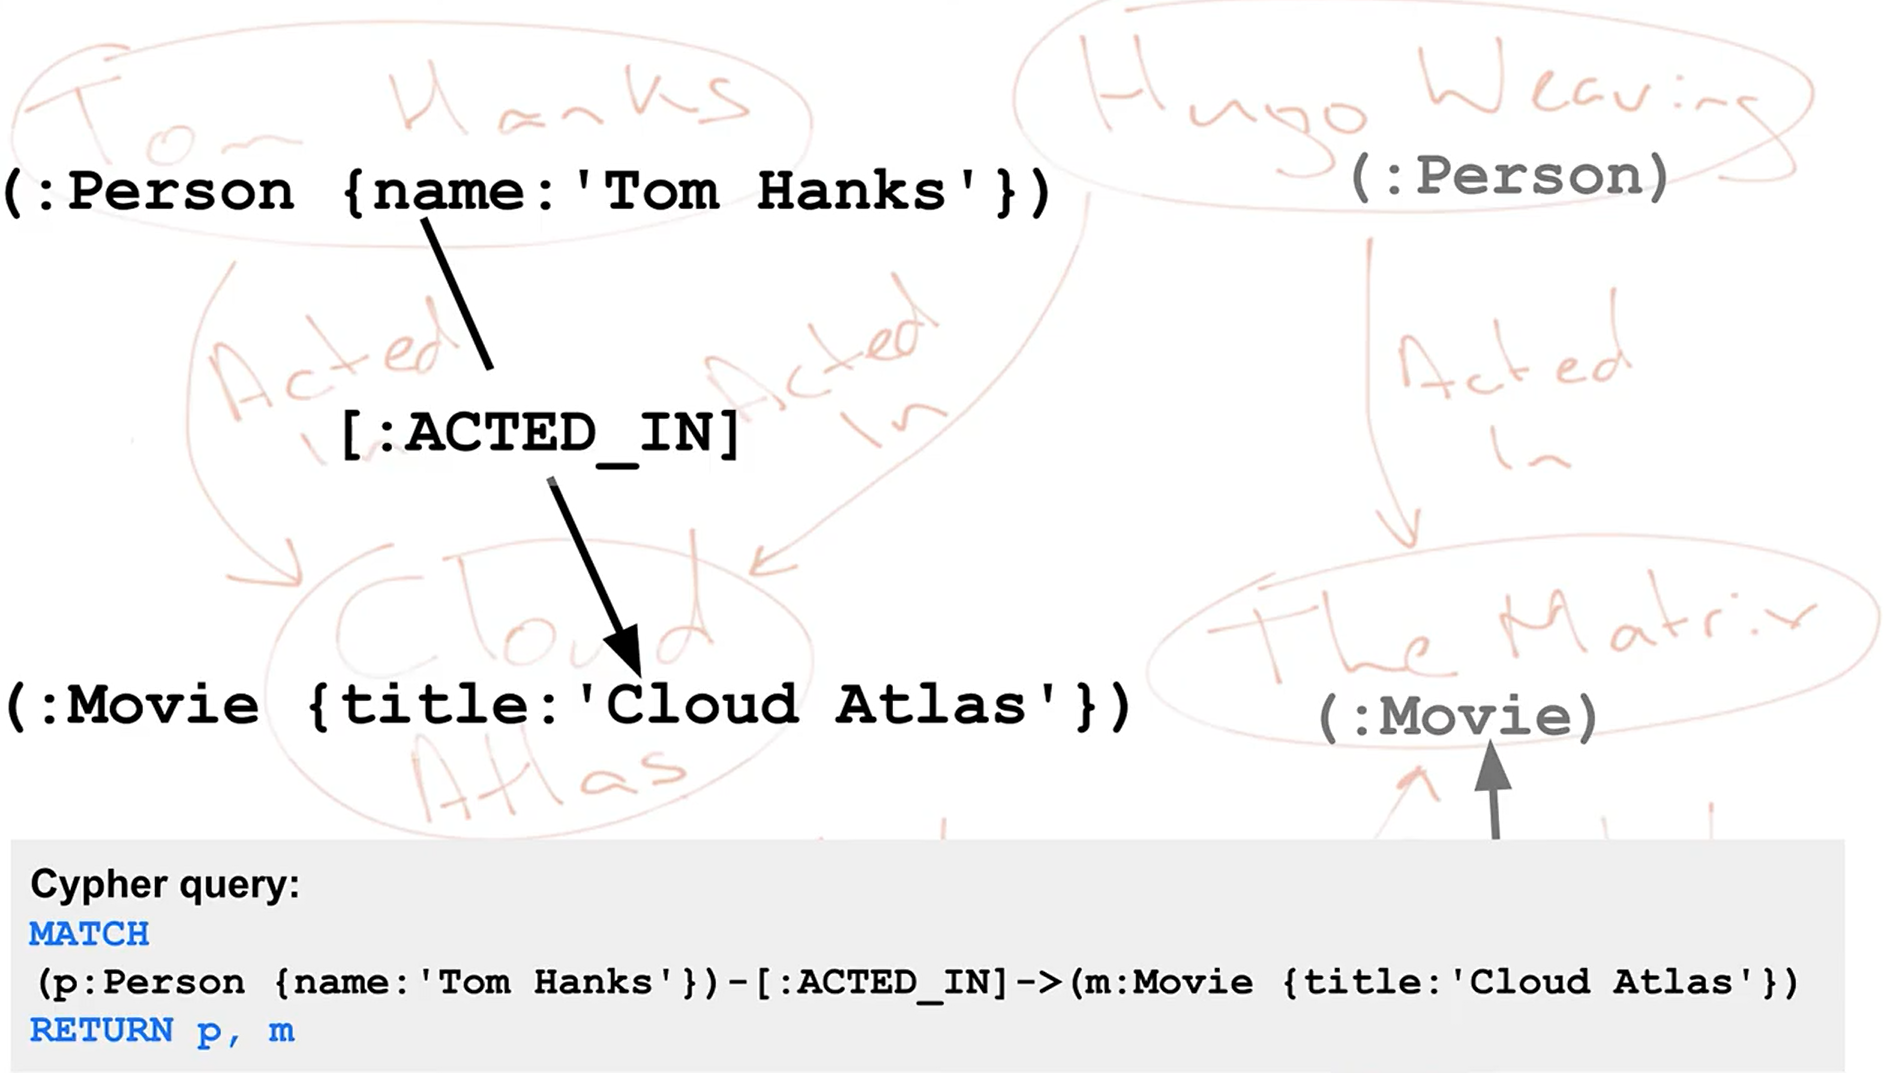
\includegraphics[width=0.5\linewidth,keepaspectratio]{neo4j64}
\end{center}	  


{\tiny (Ref: Introduction to cypher fundamentals  - neo4j)}

\end{frame}

%%%%%%%%%%%%%%%%%%%%%%%%%%%%%%%%%%%%%%%%%%%%%%%%%%%%%%%%%%%
\begin{frame}[fragile]\frametitle{Retrieval}

WHERE can be used to add logical expression, which is not possible in MATCH

\begin{center}
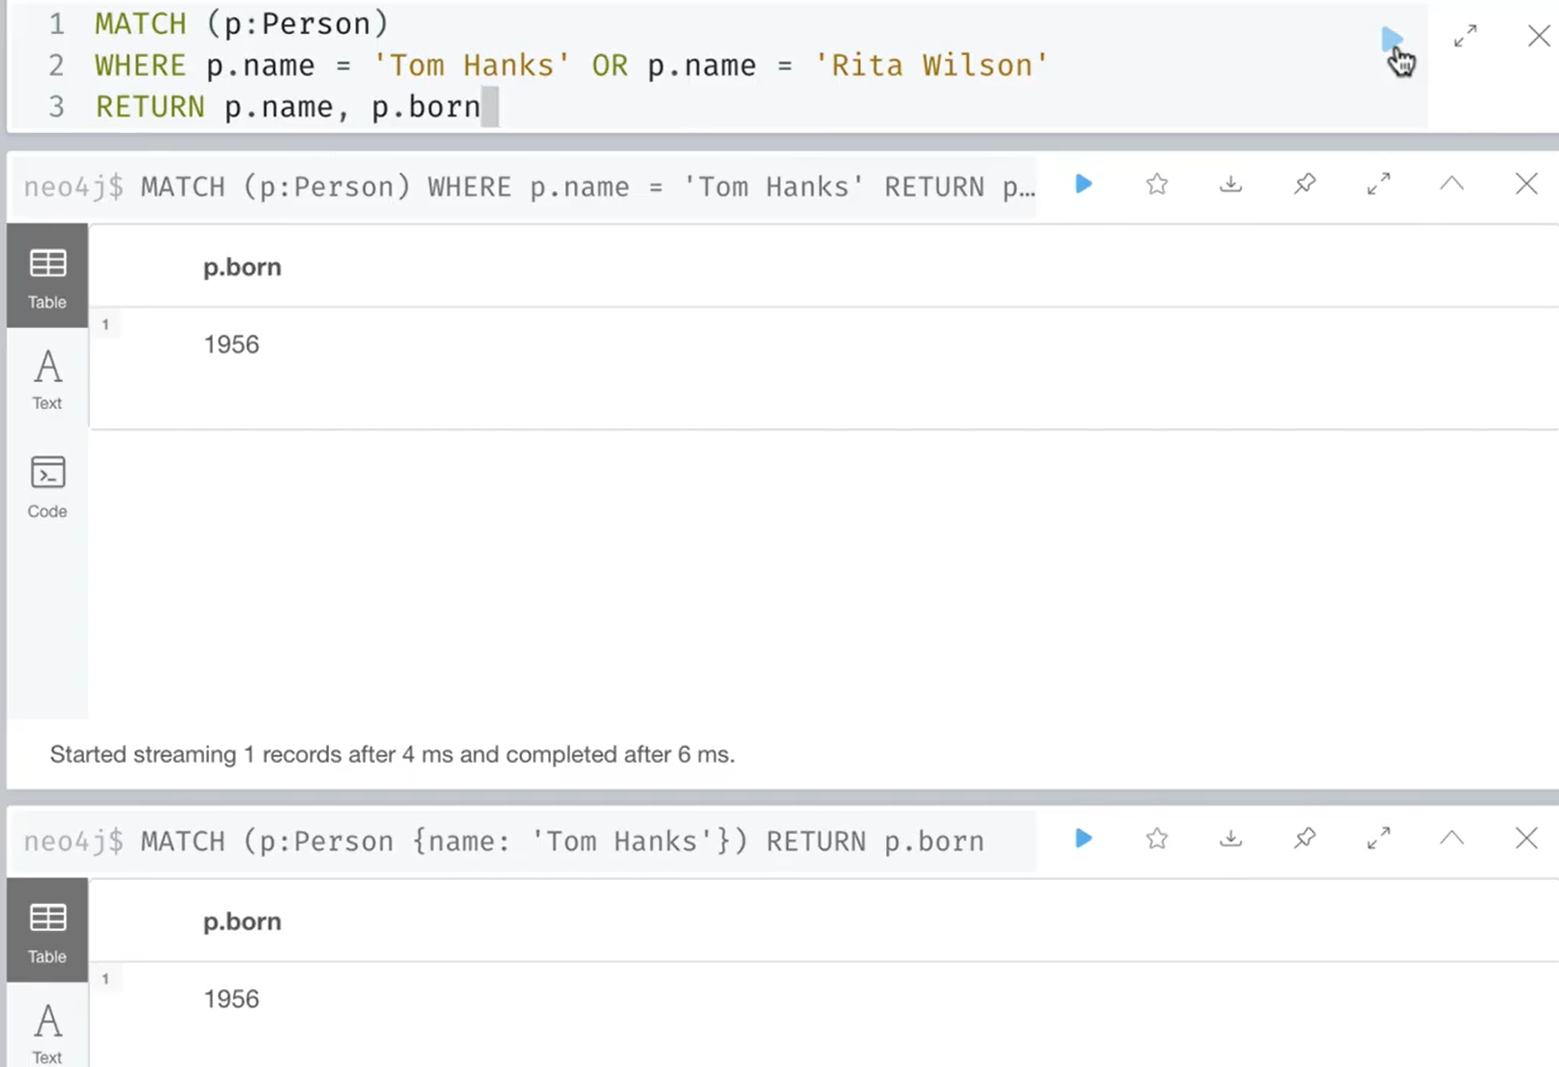
\includegraphics[width=0.5\linewidth,keepaspectratio]{neo4j65}
\end{center}	  


{\tiny (Ref: Introduction to cypher fundamentals  - neo4j)}

\end{frame}



%%%%%%%%%%%%%%%%%%%%%%%%%%%%%%%%%%%%%%%%%%%%%%%%%%%%%%%%%%%
\begin{frame}[fragile]\frametitle{MATCH}

Retrieve nodes

\begin{center}
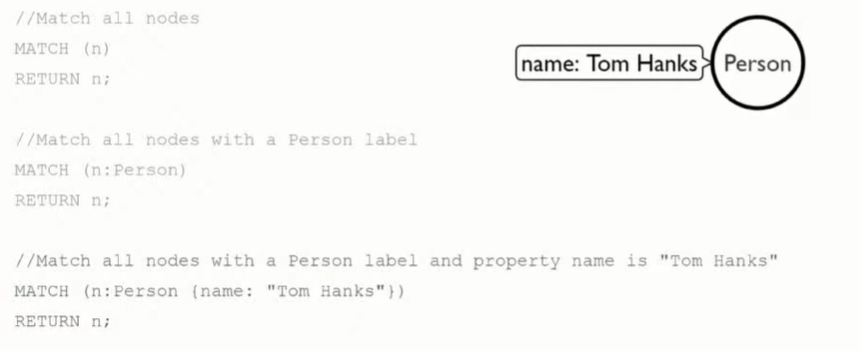
\includegraphics[width=\linewidth,keepaspectratio]{neo4j10}
\end{center}	  


{\tiny (Ref: Introduction to Neo4j - a hands-on crash course  - neo4j)}

\end{frame}

%%%%%%%%%%%%%%%%%%%%%%%%%%%%%%%%%%%%%%%%%%%%%%%%%%%%%%%%%%%
\begin{frame}[fragile]\frametitle{MATCH}

Retrieve nodes with properties

\begin{center}
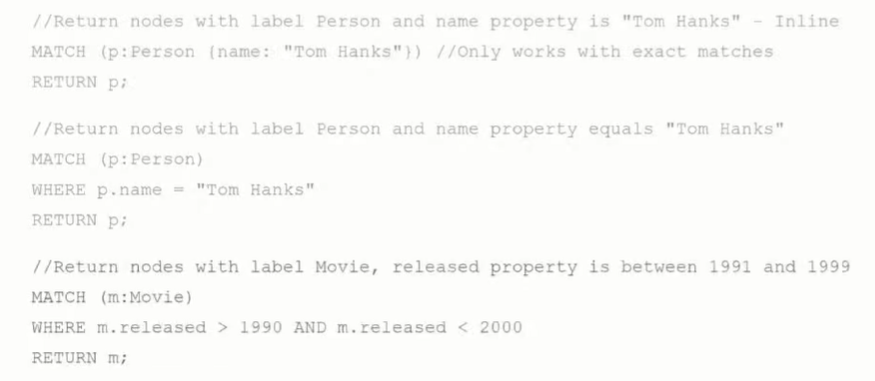
\includegraphics[width=\linewidth,keepaspectratio]{neo4j11}
\end{center}	  


{\tiny (Ref: Introduction to Neo4j - a hands-on crash course  - neo4j)}

\end{frame}

%%%%%%%%%%%%%%%%%%%%%%%%%%%%%%%%%%%%%%%%%%%%%%%%%%%%%%%%%%%
\begin{frame}[fragile]\frametitle{MATCH}

Retrieve nodes with relationships

\begin{center}
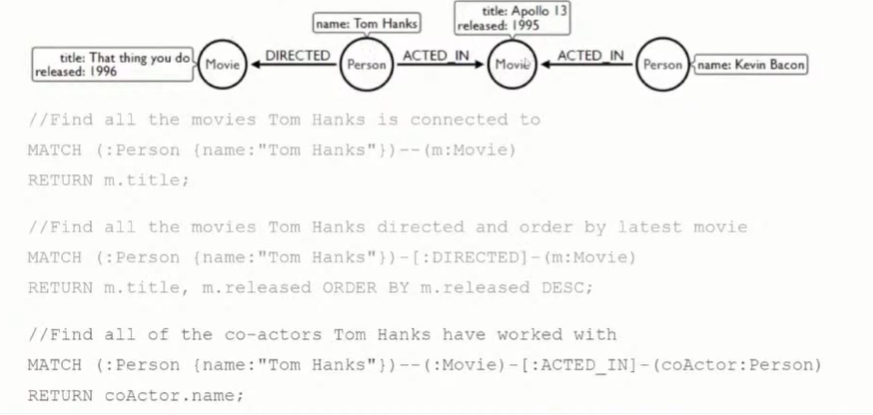
\includegraphics[width=\linewidth,keepaspectratio]{neo4j12}
\end{center}	  


{\tiny (Ref: Introduction to Neo4j - a hands-on crash course  - neo4j)}

\end{frame}

%%%%%%%%%%%%%%%%%%%%%%%%%%%%%%%%%%%%%%%%%%%%%%%%%%%%%%%%%%%
\begin{frame}[fragile]\frametitle{Retrieval}


\begin{itemize}
\item Absence of a property can also be checked in WHERE clause
\item Partial matches are allowed using STARTS\_WITH, ENDS\_WITH keywords
\item String tests are case sensitive, so better to LOWER them.
\item Check presence IN a list
\end{itemize}


\begin{center}
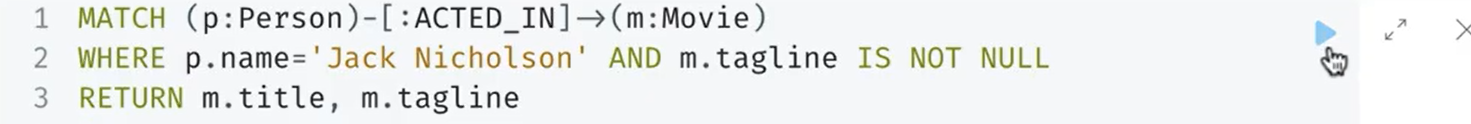
\includegraphics[width=\linewidth,keepaspectratio]{neo4j66}

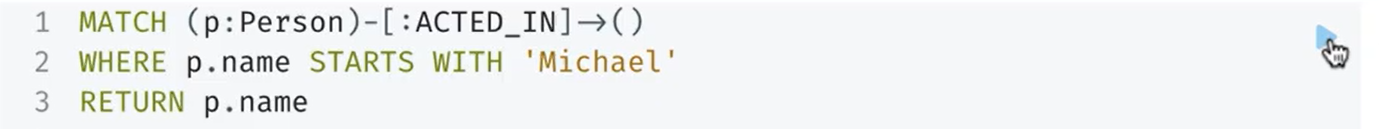
\includegraphics[width=\linewidth,keepaspectratio]{neo4j67}

\end{center}	  


{\tiny (Ref: Introduction to cypher fundamentals  - neo4j)}

\end{frame}

%%%%%%%%%%%%%%%%%%%%%%%%%%%%%%%%%%%%%%%%%%%%%%%%%%%%%%%%%%%
\begin{frame}[fragile]\frametitle{Aggregates}
No need to specify grouping key. There is no group-by statement. Other Aggregates are SUM, STDDEV, etc.


\begin{lstlisting}
// implicitly groups by p.name
MATCH (p.Person)-[:ACTED_IN]->(m:Movie)
RETURN p.name, count(*) AS numberOfMovies
\end{lstlisting}	  


\end{frame}

%%%%%%%%%%%%%%%%%%%%%%%%%%%%%%%%%%%%%%%%%%%%%%%%%%%%%%%%%%%
\begin{frame}[fragile]\frametitle{Complex Example}
A Social Recommendation

\begin{center}
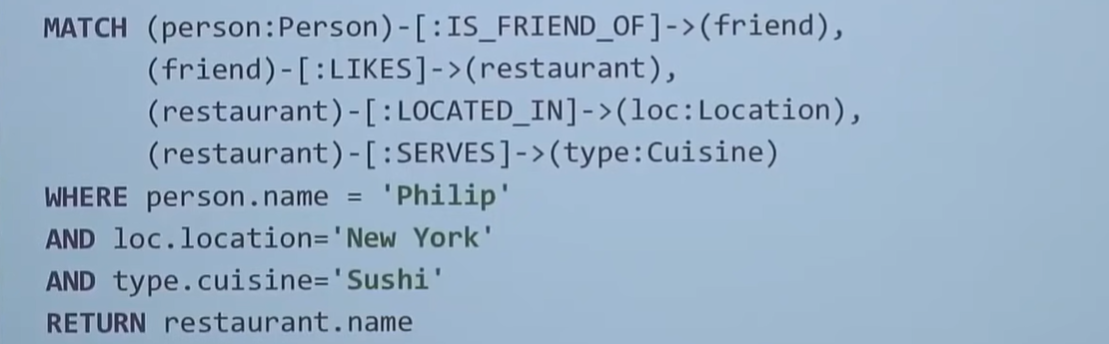
\includegraphics[width=\linewidth,keepaspectratio]{neo4j15}
\end{center}	  


{\tiny (Ref: Introduction to Neo4j and Graph Databases
 - M David Allen)}

\end{frame}



%%%%%%%%%%%%%%%%%%%%%%%%%%%%%%%%%%%%%%%%%%%%%%%%%%%%%%%%%%%
\begin{frame}[fragile]\frametitle{Complex Example}
What are the top 10 jobs for me, that are same location as I am in and also for which I have necessary qualifications?

\begin{center}
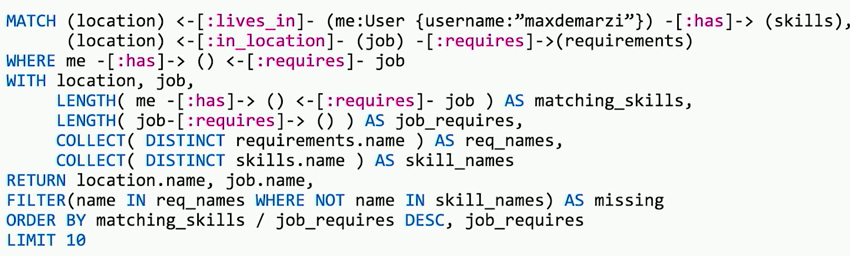
\includegraphics[width=\linewidth,keepaspectratio]{neo4j27}
\end{center}	    



{\tiny (Ref: Secret Sauce of Neo4j: Modeling and Querying Graphs
 - Max De Marzi )}

\end{frame}

%%%%%%%%%%%%%%%%%%%%%%%%%%%%%%%%%%%%%%%%%%%%%%%%%%%%%%%%%%%
\begin{frame}[fragile]\frametitle{Answer}

Partial sub-graph match

\begin{center}
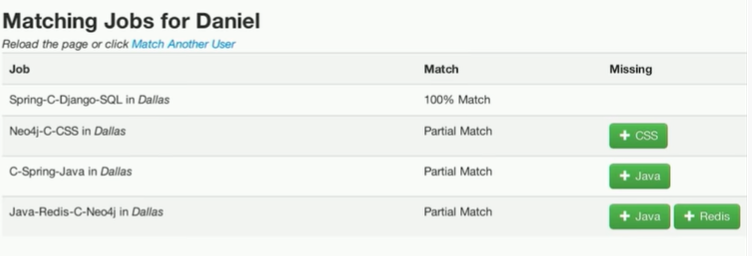
\includegraphics[width=\linewidth,keepaspectratio]{neo4j28}
\end{center}	    


{\tiny (Ref: Secret Sauce of Neo4j: Modeling and Querying Graphs
 - Max De Marzi )}

\end{frame}

%%%%%%%%%%%%%%%%%%%%%%%%%%%%%%%%%%%%%%%%%%%%%%%%%%%%%%%%%%%%%%%%%%%%%%%%%%%%%%%%%%
\begin{frame}[fragile]\frametitle{}
\begin{center}
{\Large Writing}
\end{center}
\end{frame}



%%%%%%%%%%%%%%%%%%%%%%%%%%%%%%%%%%%%%%%%%%%%%%%%%%%%%%%%%%%
\begin{frame}[fragile]\frametitle{Nodes}

\begin{itemize}
\item MERGE: Creates a new node if not present already. All subsequent calls do not do anything as node with said properties is already present.

\item CREATE: Will create multiple nodes even if nodes with similar properties are present already
\end{itemize}

\begin{center}
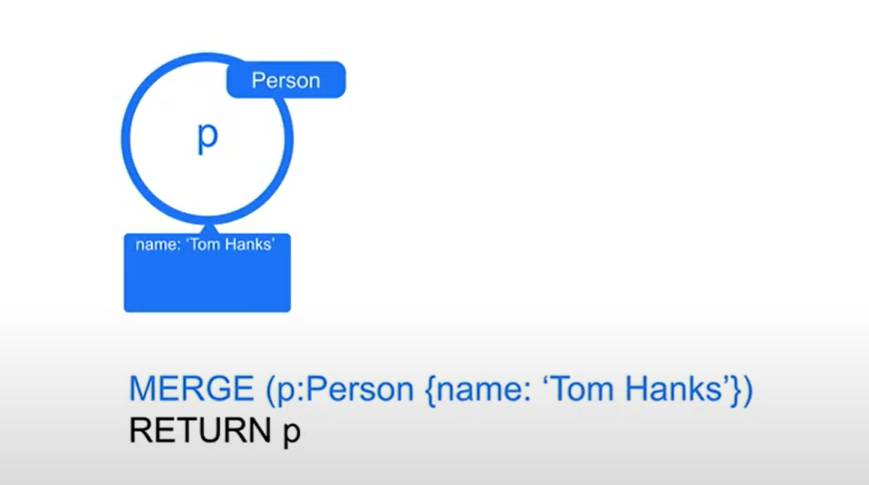
\includegraphics[width=0.5\linewidth,keepaspectratio]{neo4j68}
\end{center}	  


{\tiny (Ref: Introduction to cypher fundamentals  - neo4j)}

\end{frame}

%%%%%%%%%%%%%%%%%%%%%%%%%%%%%%%%%%%%%%%%%%%%%%%%%%%%%%%%%%%
\begin{frame}[fragile]\frametitle{Nodes}


\begin{center}
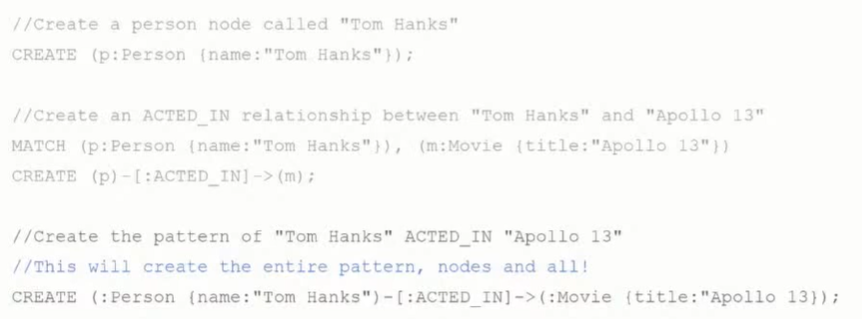
\includegraphics[width=\linewidth,keepaspectratio]{neo4j13}
\end{center}	  


{\tiny (Ref: Introduction to Neo4j - a hands-on crash course  - neo4j)}

\end{frame}


%%%%%%%%%%%%%%%%%%%%%%%%%%%%%%%%%%%%%%%%%%%%%%%%%%%%%%%%%%%
\begin{frame}[fragile]\frametitle{Relationships}

\begin{itemize}
\item First get two existing nodes between which a relationship needs to be created.
\item Same MERGE logic is there for Relationships as well.
item Relationship type must begin with ':'
\end{itemize}

\begin{center}
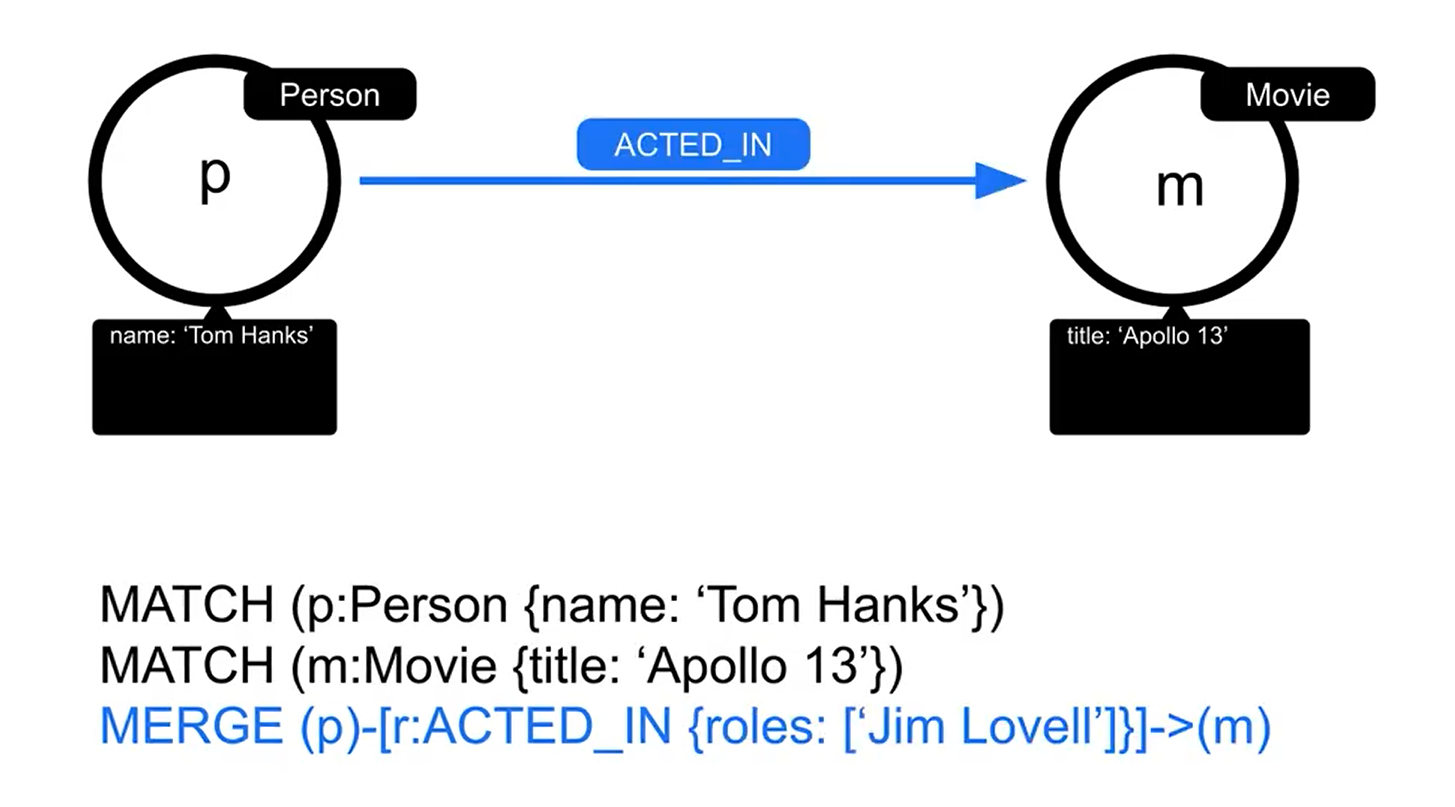
\includegraphics[width=0.8\linewidth,keepaspectratio]{neo4j69}
\end{center}	  


{\tiny (Ref: Introduction to cypher fundamentals  - neo4j)}

\end{frame}

%%%%%%%%%%%%%%%%%%%%%%%%%%%%%%%%%%%%%%%%%%%%%%%%%%%%%%%%%%%
\begin{frame}[fragile]\frametitle{Properties}

\begin{itemize}
\item Use SET to set new or existing properties
\item It can be used for both Nodes and Relationships
\item Use REMOVE to remove a property. (it should not be a primary key though)
\end{itemize}

\begin{center}
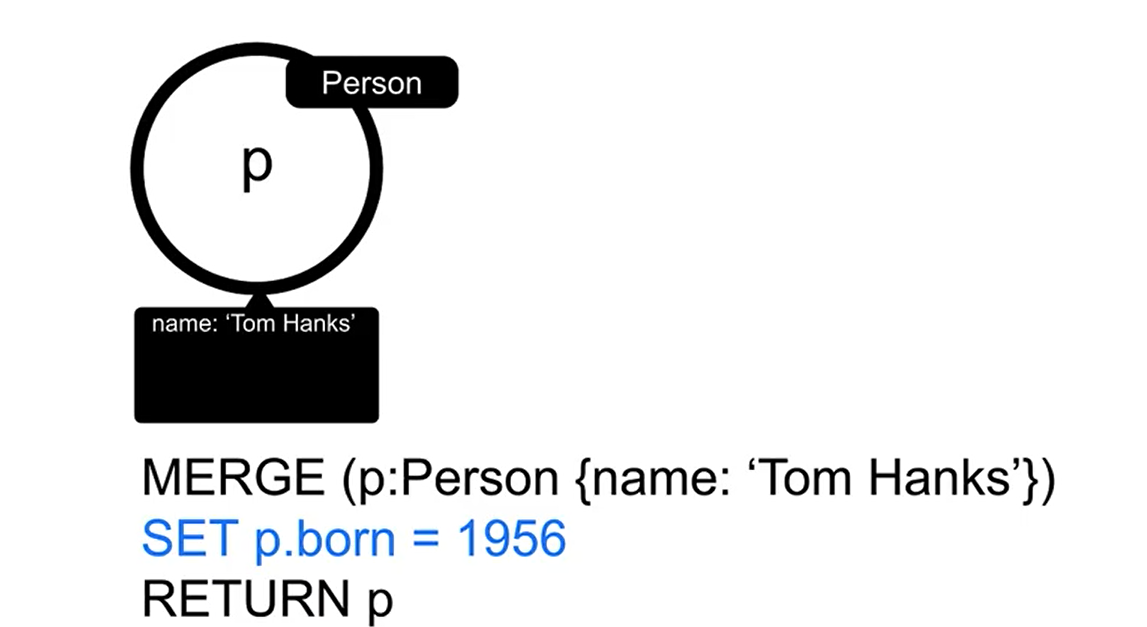
\includegraphics[width=0.5\linewidth,keepaspectratio]{neo4j70}
\end{center}	  


{\tiny (Ref: Introduction to cypher fundamentals  - neo4j)}

\end{frame}


%%%%%%%%%%%%%%%%%%%%%%%%%%%%%%%%%%%%%%%%%%%%%%%%%%%%%%%%%%%
\begin{frame}[fragile]\frametitle{Constrains}
Unique

\begin{lstlisting}
// to ensure uniqueness and fast lookups
CREATE CONSTRAINT ON (label:Label)
ASSERT label.property IS UNIQUE
\end{lstlisting}	  

\end{frame}

%%%%%%%%%%%%%%%%%%%%%%%%%%%%%%%%%%%%%%%%%%%%%%%%%%%%%%%%%%%
\begin{frame}[fragile]\frametitle{Conditionals}

\begin{itemize}
\item ON CREATE will do the SET at the time of creation, ie first time when the node is created. There ON MATCH wont run.
\item Next time, when the whole code is executed again, ON CRETAE wont run, but ON MATCH will.
\end{itemize}

\begin{center}
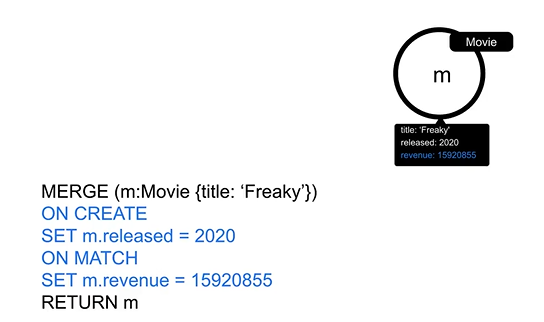
\includegraphics[width=0.5\linewidth,keepaspectratio]{neo4j71}
\end{center}	  


{\tiny (Ref: Introduction to cypher fundamentals  - neo4j)}
 

\end{frame}

%%%%%%%%%%%%%%%%%%%%%%%%%%%%%%%%%%%%%%%%%%%%%%%%%%%%%%%%%%%
\begin{frame}[fragile]\frametitle{Delete}

\begin{itemize}
\item Just get the reference to the object and delete it.
\item It can be a Node (if dangling) or a Relationship.
\item DETACH DELETE removes all relationships from the node and then DELETEs it.
\item To delete all nodes, just say \lstinline|MATCH (n) DETACH DELETE n|
\end{itemize}

\begin{center}
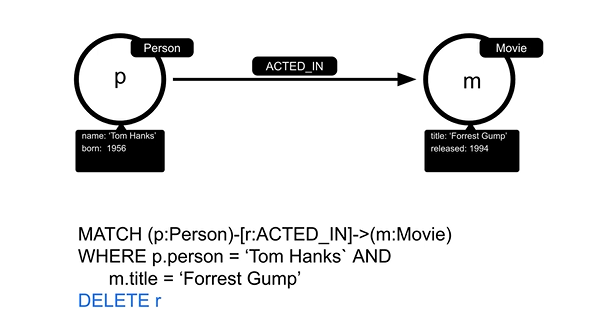
\includegraphics[width=0.5\linewidth,keepaspectratio]{neo4j72}
\end{center}	  


{\tiny (Ref: Introduction to cypher fundamentals  - neo4j)}
 

\end{frame}








